\documentclass[11pt,a4paper]{article}

% Typography
\usepackage[utf8]{inputenc}
\usepackage[T1]{fontenc}
\usepackage{mathpazo}              % Palatino for text and math
\usepackage[scaled=0.85]{berasans} % Bera Sans for sans-serif
\usepackage[scaled=0.85]{beramono} % Bera Mono for monospace
\usepackage{microtype}             % Better typographic refinement

% Layout
\usepackage[margin=1in]{geometry}
\usepackage{setspace}
\setstretch{1.15}                  % Slightly opened up line spacing
\usepackage{parskip}               % Paragraph spacing instead of indentation

% Math and tables
\usepackage{amsmath,amssymb}
\usepackage{booktabs}

% Figures
\usepackage{graphicx}
\usepackage[font=small,labelfont=bf]{caption}

% References
\usepackage[colorlinks,citecolor=blue!60!black,linkcolor=blue!60!black,urlcolor=blue!60!black]{hyperref}
\usepackage{natbib}

\title{\textbf{Feature Transport Across Grammatical Roles in Pythia-410M}}
\author{Olli Tuomi}
\date{June 2026}

\begin{document}
\maketitle

\begin{abstract}
\noindent
Cross-position information flow in transformers has been studied through subject--verb
agreement \citep{hao2023verb}, pronoun resolution circuits \citep{wang2022interpretability},
binding subspaces \citep{feng2023language}, OV singular-vector analysis
\citep{ahmad2025beyond}, and activation transport operators \citep{szablewski2025activation}.
We measure one specific mechanism---a low-rank linear map from a source token's
representation to a consuming position---across three grammatical roles in Pythia-410M-deduped.
Object channels (centered $R^2$ 0.52--0.56) are stronger than the subject channel (0.41),
despite English having no object agreement. Standard grammatical features (number, gender,
animacy) account for 27\% of the subject channel's variance; unsupervised clustering of the
remaining content recovers 7 semantic axes (place, body-part, food, person, animal, household
object, water body), each of which causally shifts next-token predictions when patched, while
matched random-direction controls do not. The transported copy is decodable at the consuming
position from layer~8 but only becomes causal at layers~20--23. All results are from one
model and one language (English).
Code and data: \url{https://github.com/EvidentSolutions/Deposit}.
\end{abstract}

%----------------------------------------------------------------------
\section{Introduction}
\label{sec:intro}
%----------------------------------------------------------------------

Cross-position information flow in transformers has been studied through several phenomena.
\citet{wang2022interpretability} identified the circuit by which GPT-2 resolves indirect
object pronouns. \citet{hao2023verb} showed that subject--verb agreement in BERT relies on a
linear encoding of subject number that can be read at the verb position.
\citet{feng2023language} found that binding in Pythia operates through low-rank subspaces.
\citet{ahmad2025beyond} decomposed OV circuits into singular-vector directions that control
gender pronoun prediction. \citet{szablewski2025activation} proposed rank-constrained
activation transport operators for tracing feature flow through the residual stream.

Most of this work examines one grammatical role at a time, typically the subject in
agreement constructions. The low-rank linear map framing---fitting a map from a source token's
representation to the consuming position and testing what features it carries---has been
applied mainly to agreement and binding. We apply the same measurement to three grammatical
roles in Pythia-410M-deduped (EleutherAI), including roles where no morphological constraint
requires cross-position transport. In principle, any position can transport features to any
other position via attention; we measure four specific source--consumer pairs out of many
possible ones, and make no claim about pairs we did not test.

We report four sets of measurements:

\begin{enumerate}
\item \textbf{Deposit channel strength by role.} Centered $R^2$ of a ridge-fit
linear map for subject$\to$verb, object$\to$pronoun, and object$\to$clause-end.
Object channels are stronger than the subject channel.

\item \textbf{Channel content.} Standard grammatical features (number, gender, animacy)
explain 27\% of the channel's variance. Unsupervised clustering of the remaining content,
followed by per-cluster causal intervention, recovers 7 additional semantic axes, all causally
validated.

\item \textbf{Timing of causal use.} The transported copy is decodable at the consuming
position from layer~8 but has no measurable causal effect on the prediction until layer~16,
reaching full effect at layers~20--23.

\item \textbf{Distributional scope.} Forcing rank-2 through rank-5 alternative tokens at the
prediction position: all 83 tested verbs across all 5 ranks respect the deposited number
constraint.
\end{enumerate}

\begin{figure}[t]
\centering
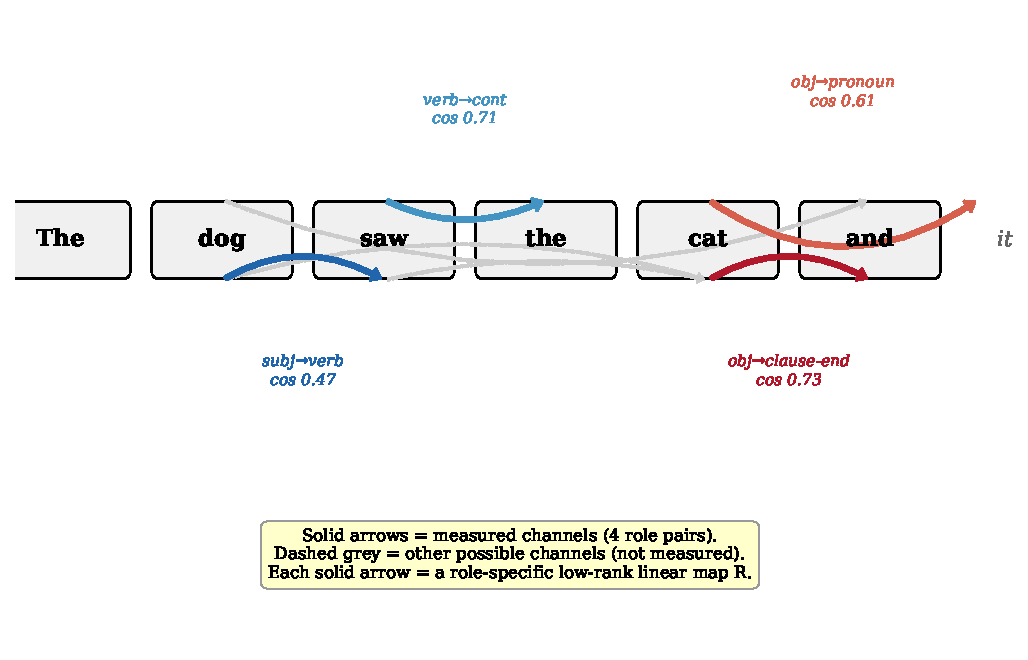
\includegraphics[width=\linewidth]{figures/fig1_schematic.pdf}
\caption{Deposit channels across grammatical roles (illustrative sentence). Solid coloured
arrows show source--consumer pairs; dashed grey arrows indicate other possible channels that
were not measured. Three noun roles (subject$\to$verb, object$\to$pronoun,
object$\to$clause-end) are quantified in Table~\ref{tab:role-comparison};
verb$\to$continuation is illustrated but not included in the centered $R^2$ analysis (it
uses a different feature battery).}
\label{fig:schematic}
\end{figure}

%----------------------------------------------------------------------
\section{Method}
\label{sec:method}
%----------------------------------------------------------------------

\textbf{Model.}\quad All experiments use Pythia-410M-deduped \citep{biderman2023pythia}, a
24-layer autoregressive transformer with $d_\mathrm{model}=1024$.

\subsection{Deposit map}
\label{sec:deposit-map}

We define a \emph{deposit map} as a linear map $R: \mathbb{R}^d \to \mathbb{R}^d$ from the
source token's residual-stream representation at a lexical layer to the consuming position's
representation at a transport layer. We use layer~8 as the lexical layer and layer~12 as the
transport layer throughout. A grid search over source layers $\{2,4,\ldots,16\}$ and consumer
layers $\{4,6,\ldots,22\}$ (Figure~\ref{fig:layer-heatmap}) shows that the centered $R^2$
forms a broad plateau: any source layer $\leq 10$ paired with any consumer layer in
$\{12,\ldots,18\}$ gives $R^2 \approx 0.33\text{--}0.38$. L8$\to$L12 ($R^2 = 0.37$) is
near the maximum (L8$\to$L14, $R^2 = 0.38$). Below consumer layer~10, the transport signal
is weak ($R^2 < 0.23$); the source layer matters little once it exceeds~2.

\begin{figure}[t]
\centering
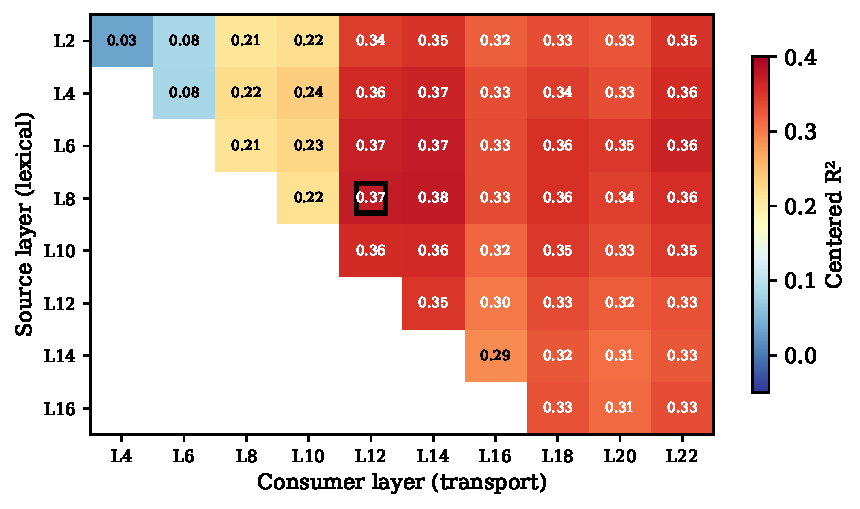
\includegraphics[width=0.85\linewidth]{figures/fig5_layer_heatmap.pdf}
\caption{Centered $R^2$ of the deposit map (subject$\to$verb) across source and consumer
layer pairs. The black square marks L8$\to$L12 (used throughout). The result is a broad
plateau: $R^2 \approx 0.33\text{--}0.38$ for source layers $\leq$10 and consumer layers
12--18.}
\label{fig:layer-heatmap}
\end{figure}

Given $N$ source words, let $X \in \mathbb{R}^{N \times d}$ be the centered lexical
representations (source token, layer~8) and $Y \in \mathbb{R}^{N \times d}$ the centered
transport representations (consuming position, layer~12). We fit $R$ by ridge regression:
\begin{equation}
R = (X^\top X + \lambda I)^{-1} X^\top Y,
\quad \lambda = 0.1 \cdot \tfrac{1}{d}\sum_j \|X_{\cdot,j}\|^2.
\end{equation}

We evaluate on held-out words (75/25 train/test split, randomized over 10 random splits) by
centered $R^2$: $R^2$ computed on mean-subtracted representations, isolating the
word-specific component from global positional structure (see \S\ref{sec:global-control}).
We also report $R^2$ restricted to the 30-dimensional channel subspace (top-30 singular
vectors of $R$) and cross-category controls where $R$ is fit on wrong-word pairings
(e.g., dog's source $\to$ chair's consumer representation).

\subsection{Feature battery}
\label{sec:feature-battery}

For each binary feature (number: singular/plural; gender: masculine/feminine; animacy:
animate/inanimate), we compute the feature direction in lexical space as the difference of
class means, and similarly in transport space. We test whether $R$ maps one to the other by
measuring $\cos(R \cdot \ell_F,\; t_F)$, where $\ell_F$ and $t_F$ are the lexical and
transport feature directions respectively.

Identity stripping is measured by $\eta^2$ of word identity (one-way ANOVA on word labels)
in the channel coordinates: $\eta^2 = 1.0$ means every word is individually distinguishable;
$\eta^2 \approx 0$ means the channel carries only abstract features.

\subsection{Discover--validate sweep}
\label{sec:discover-validate}

\begin{enumerate}
\item Extract the 30-dimensional input channel of $R$ (top-30 left singular vectors of $R$).
\item Cluster words in this space using $k$-means ($k=8$).
\item For each cluster $C$, compute a cluster direction $u_C$ (mean of cluster members minus
global mean, in channel coordinates). Measure transport cosine on held-out words:
$\cos(R \cdot u_C^\mathrm{lex},\; u_C^\mathrm{tr})$.
\item Causal test: in the frame ``The $\langle$N$\rangle$ is \underline{\hspace{1cm}}'',
patch the component of the noun's residual along $u_C$ to the cluster mean (vs.\ the
complement mean). Measure the shift in a learned category readout (mean logits for
cluster-typical continuations minus global mean logits). Compare to a matched random-direction
control (same norm, same projection magnitude, random orientation). A cluster is validated if
causal effect $> 0.3$ and $> 3\times$ the random control's effect.
\end{enumerate}

\subsection{Layer-swept causal test}
\label{sec:layer-sweep}

To test whether the \emph{transported copy} (not the source) is causal, we use the frame
``The $\langle$N$\rangle$ near the old table is a type of \underline{\hspace{1cm}}''. The
source noun is at position~1; the consuming position is the final token (7+ positions away,
past a distractor noun ``table''). We patch a discovered axis (place vs.\ object category) at
the consuming position only, at each layer from L4 to L23, and measure the shift in a
readout defined as $\mathrm{logsumexp}(\text{logits}[\text{place words}]) -
\mathrm{logsumexp}(\text{logits}[\text{object words}])$, where place words = \{city, town,
place, country, area, region\} and object words = \{object, thing, tool, device, item,
material\}. We compare to random-direction patches at the same position and layer. We use 14
place nouns and 14 object nouns.

\subsection{Forced-alternative test}
\label{sec:forced-alt}

For the prompt ``The $\langle$noun$\rangle$ near the wall'' (20 singular/plural pairs, 40
variants), we record the model's top-5 predictions. We then force each rank-$k$ token
($k=1\ldots5$) as the next token and continue greedily for 7 tokens. We check whether the
forced token is a verb that agrees in number with the subject noun.

%----------------------------------------------------------------------
\section{Results: role comparison}
\label{sec:role-comparison}
%----------------------------------------------------------------------

\subsection{Three channels measured}

We measured deposit maps for three source--consumer pairs. Stimuli follow the templates:

\begin{itemize}
\item \textbf{Subject$\to$verb:} lexical = ``The $\langle w \rangle$ near the table''
($w$ at position~1); transport = verb position in ``The $\langle w \rangle$ near the
$\langle$N2$\rangle$ $\langle$V$\rangle$'' (position~5).
\item \textbf{Object$\to$pronoun:} lexical = ``The $\langle$S$\rangle$ saw the $\langle w
\rangle$ by the wall'' ($w$ at position~4); transport = ``it'' in ``The $\langle$S$\rangle$
saw the $\langle w \rangle$ near the $\langle$N2$\rangle$ and it'' (position~9).
\item \textbf{Object$\to$clause-end:} same lexical frame; transport = ``wall'' in ``The
$\langle$S$\rangle$ saw the $\langle w \rangle$ by the wall'' (position~7).
\end{itemize}

Noun vocabulary: 112 words across 7 semantic categories (animal, person, object, place,
abstract, food, body-part), filtered to single-token items. 75/25 train/test split, averaged
over 10 random splits.

\begin{table}[t]
\centering
\caption{Deposit map quality by grammatical role (centered $R^2$, 10 random splits).}
\label{tab:role-comparison}
\begin{tabular}{lcccccc}
\toprule
Role & Centered $R^2$ & Cross-cat $R^2$ & $\Delta R^2$ & Chan.\ $R^2$ & $\eta^2$ & Eff.\ rank \\
\midrule
Subject $\to$ verb       & 0.41 & $-0.42$ & 0.83 & 0.94 & 0.16 & 32 \\
Object $\to$ pronoun     & 0.52 & $-0.33$ & 0.85 & 0.96 & 0.30 & 33 \\
Object $\to$ clause-end  & 0.56 & $-0.65$ & 1.22 & 0.95 & 0.55 & 36 \\
\bottomrule
\end{tabular}

\smallskip\small
Centered $R^2$: ridge regression on mean-subtracted (word-specific) representations, 75/25
split, averaged over 10 random splits. Cross-cat $R^2$: same map fitted on cross-category
word pairings (dog$\to$chair); negative values mean the wrong-word map hurts prediction.
$\Delta R^2$ = matched $-$ cross-category. Chan.\ $R^2$: $R^2$ restricted to the 30-dim
channel subspace (top-30 singular vectors of $R$). $\eta^2$ = ANOVA on word identity (1.0 =
identity preserved). Verb$\to$continuation omitted (different feature battery; see text).
\end{table}

Table~\ref{tab:role-comparison} shows the results using centered $R^2$ (word-specific
component only; see \S\ref{sec:global-control} for why uncentered cosine is not appropriate).
Object channels have higher centered $R^2$ than the subject channel:
object$\to$clause-end (0.56) and object$\to$pronoun (0.52) vs.\ subject$\to$verb (0.41).
English has no morphological object agreement; the transport exists without morphological
pressure. All cross-category $R^2$ values are strongly negative ($-0.33$ to $-0.65$),
confirming that the map captures word-specific content, not global structure.

Within the 30-dimensional channel subspace (top-30 singular vectors of $R$), $R^2$ rises to
0.94--0.96 for all roles. The ``low'' full-space $R^2$ (0.41--0.56) reflects the channel's
low dimensionality relative to the 1024-dim residual stream, not weak transport.

Identity stripping varies by role. Subject$\to$verb strips most aggressively ($\eta^2 =
0.16$): 84\% of word-identity information is removed, leaving only abstract features.
Object$\to$clause-end preserves more identity ($\eta^2 = 0.55$), consistent with the
specific object constraining the continuation more than the specific noun constrains
agreement.

Cross-role transfer fails: $R_\mathrm{subj}$ applied to object data gives centered $R^2$
near zero. The maps are role-specific instantiations of the same architectural mechanism.

\label{sec:global-control}
\paragraph{Global-structure control.}
The uncentered held-out cosine (used in prior work) conflates word-specific
transport with global residual-stream structure shared between positions. To separate these,
we ran two controls using 74 words across 7 semantic categories (10 random splits each).

\emph{Uncentered cosine} (used in prior work on deposit maps) is dominated by
global structure: matched = 0.477, cross-category swap (dog$\to$chair, king$\to$river) =
0.474, fixed-word (all sentences contain ``dog'') = 0.504. The word-specific increment in
this metric is near zero.

\emph{Centered $R^2$} (mean-subtracted across words, isolating the word-varying component)
tells a different story: matched $R^2 = 0.43$, cross-category $R^2 = -0.30$ (a map fit on
wrong pairings actively hurts prediction of the word-specific component). The word-specific
$\Delta R^2$ is 0.73. This holds across context lengths: with a 25-token filler prefix,
$\Delta R^2 = 0.85$; with a 45-token prefix, $\Delta R^2 = 0.69$.

The deposit map captures genuine word-specific transport, but the uncentered held-out cosine
is not an appropriate metric for measuring it---it is swamped by the ${\sim}1000$-dimensional
global structure. The feature battery (Table~\ref{tab:feature-transport}) and the causal
validation (\S\ref{sec:channel-content}, \S\ref{sec:timing}) are the appropriate evidence.
The centered $R^2$ of the map (0.43) is a better measure of word-specific transport quality,
though it too is influenced by the choice of regularisation and train/test split.

\subsection{Feature re-encoding through one map}

A single ridge-fit map $R$ (not fitted per feature) reproduces the transport of all three
tested feature directions:

\begin{table}[h]
\centering
\caption{Per-feature transport cosine $\cos(R \cdot \ell_F,\; t_F)$ by role. The map $R$ is
fit per role on word-level representations (not per feature). Raw cos = cosine between
lexical and transport feature directions without the map.}
\label{tab:feature-transport}
\begin{tabular}{lccc}
\toprule
Feature & Subj$\to$verb & Obj$\to$pronoun & Obj$\to$clause-end \\
\midrule
Number   & 0.77 {\small(raw 0.23)} & 0.93 & 0.83 \\
Gender   & 0.80 {\small(raw 0.30)} & 0.75 & 0.76 \\
Animacy  & 0.94 {\small(raw 0.14)} & 0.97 & 0.93 \\
\bottomrule
\end{tabular}

\smallskip\small
Raw cosines (without the map) shown for subject$\to$verb only; comparable values for the
other roles.
\end{table}

All three noun-role channels transport all three features (cosine 0.75--0.97). Without the
map, the cosines are low (0.14--0.30 for subject$\to$verb); the map raises them substantially.
The map has effective rank $\approx 30$ out of 1024 dimensions: a low-rank projection that
re-encodes prediction-relevant features while discarding lexical identity.

\begin{figure}[t]
\centering
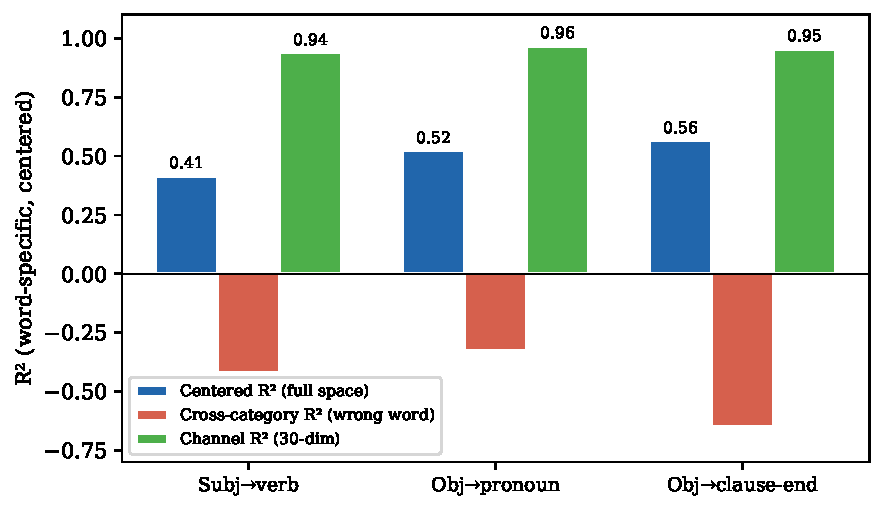
\includegraphics[width=\linewidth]{figures/fig2_role_comparison.pdf}
\caption{Word-specific transport quality by role. Blue: centered $R^2$ on the full 1024-dim
space. Red: cross-category control (map fit on wrong-word pairings; negative values confirm
word-specificity). Green: $R^2$ restricted to the 30-dim channel subspace (top-30 singular
vectors of $R$).}
\label{fig:role-comparison}
\end{figure}

%----------------------------------------------------------------------
\section{Results: channel content beyond grammatical features}
\label{sec:channel-content}
%----------------------------------------------------------------------

\subsection{Named features cover 27\%}

We projected the lexical representations of 81 nouns (spanning 7 coarse semantic categories:
person, animal, object, abstract, place, body-part, food) into the 30-dimensional input
channel of $R$ (top-30 left singular vectors). Standard grammatical features (number, gender,
animacy, person-vs-animal, concrete-vs-abstract) explain 27\% of the channel's variance. The
remaining 73\% carries structure not captured by these features.

\subsection{Unsupervised clustering}

$k$-means clustering ($k=8$) on the channel-projected words recovers semantic groupings
(Table~\ref{tab:discovered-axes}). We validated each cluster using the discover--validate
procedure described in \S\ref{sec:discover-validate}.

\begin{table}[t]
\centering
\caption{Discovered semantic axes: transport quality and causal validation.}
\label{tab:discovered-axes}
\begin{tabular}{llcccc}
\toprule
Cluster & Example words & $n$ & Transport cos & Causal effect & Random effect \\
\midrule
Food       & bread, seed, apple, rice   & 17 & 0.83 & 79.8  & $-0.07$ \\
Person     & teacher, actor, king       & 16 & 0.93 & 139.0 & $\phantom{-}0.02$ \\
Body/abstr.\ & heart, bone, faith, head & 35 & 0.91 & 61.2  & $-0.02$ \\
Household  & plate, cup, box, desk      & 10 & ---  & 60.9  & $\phantom{-}0.01$ \\
Animal     & dog, frog, deer, wolf      & 19 & 0.76 & 89.8  & $\phantom{-}0.13$ \\
Place      & country, harbor, forest    & 15 & 0.85 & 96.6  & $\phantom{-}0.01$ \\
Water      & lake, river, grass         &  3 & ---  & 103.2 & $-0.11$ \\
\bottomrule
\end{tabular}

\smallskip\small
Transport cos: $\cos(R \cdot u_C^\mathrm{lex},\; u_C^\mathrm{tr})$ on held-out words.
Causal effect: shift in category readout when patching the cluster axis at the noun position.
Random effect: same measurement with a matched random-direction control. ``---'' = too few
held-out words for reliable transport estimate. $k$-means with $k=8$ produced 7 non-empty
clusters; all 7 pass validation (causal effect $> 0.3$ and $> 3\times$ random).
\end{table}

One cluster slot (cluster~3) was empty after $k$-means. All 7 non-empty clusters both
transport through $R$ (held-out cosine 0.76--0.93) and shift the next-token distribution
when patched, while the matched random-direction control does not.

\subsection{Detailed validation: place and body-part axes}

Two discovered axes were examined with separate causal tests using dedicated stimulus frames
and readout word sets:

\begin{itemize}
\item \textbf{Place axis} (frame: ``The $\langle$N$\rangle$ is a type of
\underline{\hspace{1cm}}''): transport cosine 0.85, causal effect $+4.16$ on the
place-vs-object readout, random control $-0.002$.
\item \textbf{Body-part axis} (frame: ``The $\langle$N$\rangle$ is a part of the
\underline{\hspace{1cm}}''): transport cosine 0.89, causal effect $+2.76$, random $-0.005$.
\end{itemize}

These transport cosines are comparable to the hand-named animacy axis (${\sim}0.94$). The
channel carries semantic category information at the same fidelity as grammatical features.

\begin{figure}[t]
\centering
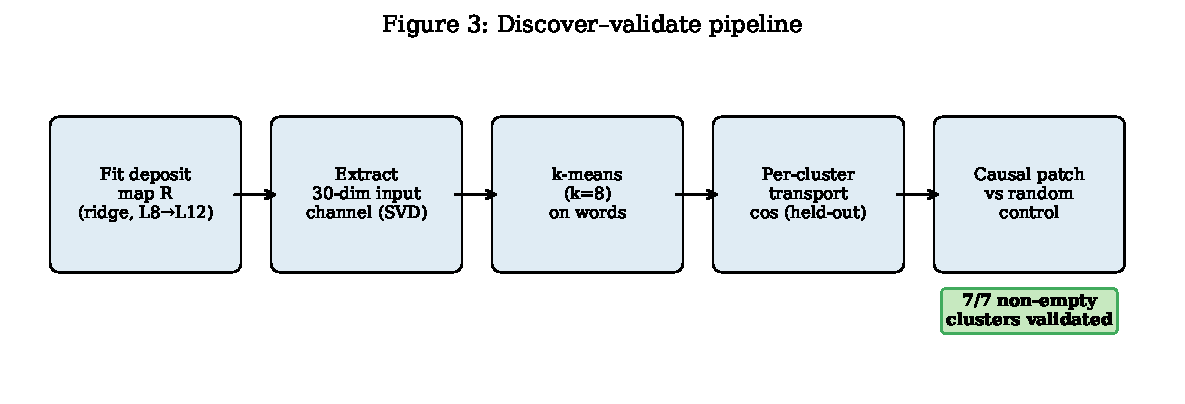
\includegraphics[width=\linewidth]{figures/fig3_pipeline.pdf}
\caption{The discover--validate pipeline. Words are projected into the 30-dimensional input
channel of $R$ (via SVD), clustered with $k$-means, and each cluster is tested for
(a)~transport through $R$ on held-out words and (b)~causal effect on next-token predictions
vs.\ a matched random-direction control. All 7 non-empty clusters passed validation.}
\label{fig:pipeline}
\end{figure}

%----------------------------------------------------------------------
\section{Results: the transported copy becomes causal late}
\label{sec:timing}
%----------------------------------------------------------------------

The transported copy is decodable at the consuming position from layer~8 (probe accuracy
$\approx 1.0$ from the role deposit tests). To measure when it becomes \emph{causal}, we
patched the place-axis component at the consuming position (final token in ``The
$\langle$N$\rangle$ near the old table is a type of \underline{\hspace{1cm}}'') at each
layer from L4 to L23. The source noun is at position~1; only the transported copy exists at
the consuming position.

\begin{table}[t]
\centering
\caption{Causal effect of patching the place axis at the consuming position, by layer.}
\label{tab:layer-sweep}
\begin{tabular}{lcc}
\toprule
Layer & Causal effect & Random effect \\
\midrule
L4  & 0.05 & $\approx 0$ \\
L8  & 0.10 & 0.001 \\
L12 & 0.82 & $-0.003$ \\
L16 & 2.19 & $-0.001$ \\
L20 & 4.28 & $-0.003$ \\
L23 & 4.48 & $-0.004$ \\
\midrule
Source noun (L8) & 3.19 & $\approx 0$ \\
\bottomrule
\end{tabular}

\smallskip\small
Causal effect: shift in $\mathrm{logsumexp}(\text{logits}[\text{place words}]) -
\mathrm{logsumexp}(\text{logits}[\text{object words}])$ when patching the place-axis
component to the place-class mean vs.\ the object-class mean. Random effect: same
measurement with a matched random direction. Source noun row: patching the place axis at the
noun's own position at L8.
\end{table}

The causal effect is near zero at L8 where the feature is decodable, and reaches its maximum
at L20--23---the layers where the model writes the prediction
(Table~\ref{tab:layer-sweep}). The source noun's features are causal early (effect 3.19 at
L8), confirming the information exists at the source; the model reads the transported copy
only at the late write-out.

A single-layer causal test at L8 (where the feature is readable) would find no effect and
conclude the transported copy is not used. The layer sweep shows it \emph{is} used, but
later (Figure~\ref{fig:layer-sweep}).

\begin{figure}[t]
\centering
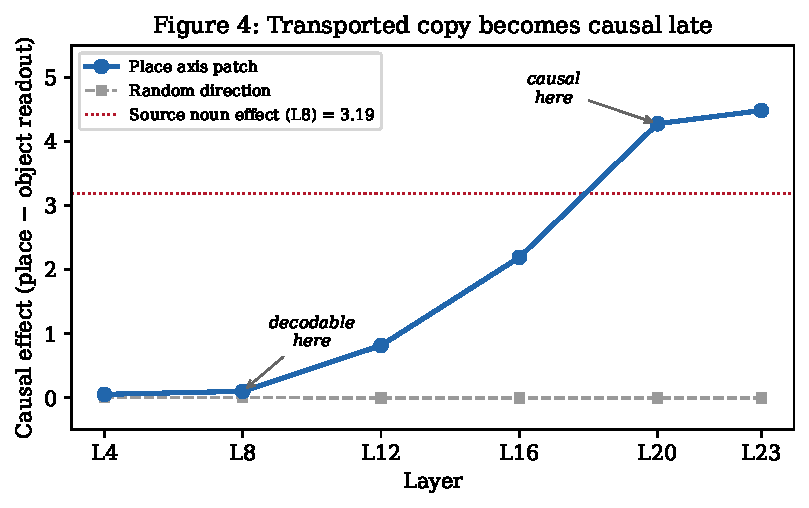
\includegraphics[width=0.85\linewidth]{figures/fig4_layer_sweep.pdf}
\caption{Causal effect of patching the place axis at the consuming position, by layer. The
feature is decodable from L8 but has near-zero causal effect until L16, reaching full effect
at L20--23. The dotted line shows the effect of patching the source noun directly at L8.
The random-direction control (dashed grey) is near zero throughout.}
\label{fig:layer-sweep}
\end{figure}

%----------------------------------------------------------------------
\section{Results: the deposit constrains beyond the top prediction}
\label{sec:forced-alt-results}
%----------------------------------------------------------------------

For 40 prompts (``The $\langle$noun$\rangle$ near the wall'', 20 singular/plural pairs), we
forced the model's rank-1 through rank-5 predictions as the next token and continued
greedily for 7~tokens. Of the 200 forced continuations (40 prompts $\times$ 5 ranks), many
forced tokens are punctuation or prepositions (commas, periods, ``of''), not verbs.
Restricting to forced tokens that are verbs: rank-1 produced 26 verbs (26/26 agree in
number), rank-2 produced 26 (26/26), rank-3 produced 16 (16/16), rank-4 produced 8 (8/8),
rank-5 produced 7 (7/7). In total, 83/83 verbs across all ranks respect number agreement
with the subject noun. P(rank-1) = 0.14, P(rank-2) = 0.10. Cascades diverge immediately
(0\% token overlap at $t+1$ between rank-1 and rank-2 continuations) but all verbs obey the
number constraint.

%----------------------------------------------------------------------
\section{Related work}
\label{sec:related}
%----------------------------------------------------------------------

\paragraph{OV abstraction and low-rank structure.}
\citet{elhage2021mathematical} described OV matrices as low-rank linear maps in their
mathematical framework for transformer circuits. \citet{xiao2024dcmha} showed that an OV
circuit can transform an object token to its superclass (Appendix~G.1).
\citet{feucht2025vector} demonstrated that concept-induction heads strip token identity while
preserving abstract attributes. The deposit map measured here is an instance of this known
structure. What we add is the cross-role comparison and the channel content analysis.

\paragraph{Pronoun resolution.}
The indirect object identification circuit \citep{wang2022interpretability} is the
most-studied cross-position circuit in mechanistic interpretability. It is framed as circuit
discovery rather than feature transport, but studies the same underlying phenomenon.
\citet{dunefsky2024observable} used pronoun prediction as a test case for feature vectors.

\paragraph{Binding subspaces.}
\citet{feng2023language} found that binding in Pythia operates through low-rank subspaces.
\citet{dai2024representational} localized Ordering~ID representations that causally determine
binding behavior. We measure the same kind of mechanism for additional roles (object, verb)
and find that maps are role-specific (applying one role's map to another's data fails).

\paragraph{OV singular vectors.}
\citet{ahmad2025beyond} decomposed OV circuits into singular-vector directions that control
gender pronoun prediction, showing that individual heads implement multiple overlapping
subfunctions aligned with distinct singular directions.

\paragraph{Activation transport operators.}
\citet{szablewski2025activation} proposed rank-constrained linear maps for tracing feature
transport through the residual stream. Their framework is general; our measurement is
role-specific and includes causal validation of discovered channel content.

\paragraph{Agreement probing.}
\citet{hao2023verb} traced subject number transport in BERT. \citet{hernandez2024linearity}
studied factual associations as linear relational embeddings. Our measurements extend to
roles without morphological agreement.

\paragraph{Causal probing.}
Activation patching \citep{meng2022locating} and automated circuit discovery
\citep{conmy2023towards} are standard tools. The layer sweep in \S\ref{sec:timing} shows
that a single-layer causal test can miss a late-used transported signal.

\paragraph{Feature discovery.}
\citet{engels2024not} characterized SAE reconstruction error as mostly linear. Our
discover--validate sweep uses unsupervised clustering on the deposit channel's input space
rather than SAE decomposition.

%----------------------------------------------------------------------
\section{Discussion}
\label{sec:discussion}
%----------------------------------------------------------------------

\paragraph{Summary of findings.}
In Pythia-410M, the low-rank linear map that transports features from source tokens to
consuming positions exists for objects, not only for subject--verb agreement.
Object channels have higher centered $R^2$ than the subject channel (0.52--0.56 vs.\ 0.41).
The subject channel carries features that are mostly grammatical (feature-subspace $R^2$ =
0.86); the object channel carries richer content (feature-subspace $R^2$ = 0.43), consistent
with the object's semantic identity mattering for prediction beyond agreement features.
The channel carries semantic category information beyond standard grammatical features, and
the transported copy becomes causal only at the model's late layers.

\paragraph{Limitations.}
All results are from one model (Pythia-410M-deduped) and one language (English). We do not
know whether these patterns hold in other architectures or at other scales. The deposit map
is fit by ridge regression on a vocabulary of 112 nouns for the role comparison and 81 nouns
for the channel content analysis; a larger or more diverse vocabulary might change the
effective rank or identity-stripping measurements.

The linear map $R$ captures only the linear component of cross-position transport. Any
nonlinear composition by attention heads before writing would be missed. We extract the
top-30 singular vectors of $R$ for the channel content analysis; low-variance directions
outside this subspace could carry additional features. The feature battery (5 hand-specified
features plus 7 discovered clusters from $k$-means with $k=8$) does not exhaustively
characterize the channel's content. The layer-pair sweep
(Figure~\ref{fig:layer-heatmap}) shows that L8$\to$L12 is near-optimal and the result is
robust across a broad range of layer pairs, but the channel content analysis and causal tests
were only run at this one pair.

We do not trace which attention heads compute the deposit or how the QK routing selects the
source token. The causal tests measure shifts in category-level predictions (e.g., ``place
words become more probable''); we do not trace downstream effects on full generation. The
causal tests use specific syntactic frames (``The N is a type of \underline{\hspace{1cm}}'');
results may differ in other frames.

\paragraph{Relation to known structure.}
The deposit map is an instance of the low-rank OV abstraction described in prior work.
Cross-position information flow has been studied through several other phenomena (IOI,
binding, activation transport operators; see \S\ref{sec:related}). The measurements that
are, to our knowledge, not previously reported are: the cross-role comparison with proper
controls for global structure (object channels stronger than the subject channel in centered
$R^2$), the channel content beyond grammatical features (73\% unnamed, with per-axis causal
validation), and the layer gap between decodability and causal use of the transported copy.
The finding that uncentered cosine---used in prior deposit-map work---is dominated by global
positional structure may be relevant to other studies using this metric.

%----------------------------------------------------------------------
\section*{Acknowledgements}
%----------------------------------------------------------------------

This research was conducted with Claude (Anthropic) as a collaborative tool.
The human author directed all research questions, validated all claims, and
takes full responsibility. Code and data at
\url{https://github.com/EvidentSolutions/Deposit}.

%----------------------------------------------------------------------
\appendix
\section{Human--AI collaborative research protocol}
\label{sec:protocol}
%----------------------------------------------------------------------

This research was conducted through iterative conversation with Claude
(Anthropic). The human author directed research questions, validated outputs,
and approved all claims. Claude conducted technical execution including code
writing, experiment design, and statistical analysis. The human author takes
full responsibility for all scientific claims.

%----------------------------------------------------------------------
\bibliographystyle{plainnat}
\begin{thebibliography}{99}

\bibitem[Ahmad et~al.(2025)]{ahmad2025beyond}
Ahmad, A., Joshi, A., and Modi, A.
\newblock Beyond components: Singular vector-based interpretability of transformer circuits.
\newblock In \emph{Advances in NeurIPS}, 2025.

\bibitem[Biderman et~al.(2023)]{biderman2023pythia}
Biderman, S., Schoelkopf, H., Anthony, Q., et~al.
\newblock Pythia: A suite for analyzing large language models across training and scaling.
\newblock In \emph{Proceedings of ICML}, 2023.

\bibitem[Conmy et~al.(2023)]{conmy2023towards}
Conmy, A., Mavor-Parker, A.~N., Lynch, A., Heimersheim, S., and Garriga-Alonso, A.
\newblock Towards automated circuit discovery for mechanistic interpretability.
\newblock In \emph{Advances in NeurIPS}, 2023.

\bibitem[Dai et~al.(2024)]{dai2024representational}
Dai, Q., Heinzerling, B., and Inui, K.
\newblock Representational analysis of binding in language models.
\newblock \emph{arXiv preprint arXiv:2409.05448}, 2024.

\bibitem[Dunefsky and Cohan(2024)]{dunefsky2024observable}
Dunefsky, J. and Cohan, A.
\newblock Observable propagation: Uncovering feature vectors in transformers.
\newblock In \emph{Proceedings of ICML}, 2024.

\bibitem[Elhage et~al.(2021)]{elhage2021mathematical}
Elhage, N., Nanda, N., Olsson, C., et~al.
\newblock A mathematical framework for transformer circuits.
\newblock \emph{Transformer Circuits Thread}, 2021.

\bibitem[Engels et~al.(2024)]{engels2024not}
Engels, J., Liao, I., Michaud, E.~J., Gurnee, W., and Tegmark, M.
\newblock Not all language model features are linear.
\newblock \emph{arXiv preprint arXiv:2405.14860}, 2024.

\bibitem[Feng and Steinhardt(2023)]{feng2023language}
Feng, G. and Steinhardt, J.
\newblock How do language models bind entities in context?
\newblock \emph{arXiv preprint arXiv:2310.17191}, 2023.

\bibitem[Feucht et~al.(2025)]{feucht2025vector}
Feucht, S., Wallace, B.~C., and Bau, D.
\newblock Vector arithmetic in concept and token subspaces.
\newblock \emph{arXiv preprint arXiv:2511.18162}, 2025.

\bibitem[Hao and Linzen(2023)]{hao2023verb}
Hao, S. and Linzen, T.
\newblock Verb conjugation in transformers is determined by linear encodings of subject number.
\newblock \emph{arXiv preprint arXiv:2310.15151}, 2023.

\bibitem[Hernandez et~al.(2024)]{hernandez2024linearity}
Hernandez, E., Sharma, A.~S., Haklay, T., Meng, K., Wattenberg, M., Andreas, J.,
Belinkov, Y., and Bau, D.
\newblock Linearity of relation decoding in transformer language models.
\newblock In \emph{Proceedings of ICLR}, 2024.

\bibitem[Meng et~al.(2022)]{meng2022locating}
Meng, K., Bau, D., Mitchell, A., and Belinkov, Y.
\newblock Locating and editing factual associations in {GPT}.
\newblock In \emph{Advances in NeurIPS}, 2022.

\bibitem[Szablewski and Masiak(2025)]{szablewski2025activation}
Szablewski, A. and Masiak, K.
\newblock Activation transport operators.
\newblock \emph{arXiv preprint arXiv:2508.17540}, 2025.

\bibitem[Wang et~al.(2023)]{wang2022interpretability}
Wang, K., Variengien, A., Conmy, A., Shlegeris, B., and Steinhardt, J.
\newblock Interpretability in the wild: A circuit for indirect object identification in
{GPT-2} small.
\newblock In \emph{Proceedings of ICLR}, 2023.

\bibitem[Xiao et~al.(2024)]{xiao2024dcmha}
Xiao, D., Meng, Q., Li, S., and Yuan, X.
\newblock Improving transformers with dynamically composable multi-head attention.
\newblock In \emph{Proceedings of ICML}, 2024.

\end{thebibliography}

\end{document}
